\documentclass[aspectratio=169]{beamer}
\usetheme{simple}

\RequirePackage[l2tabu, orthodox]{nag}


% \usepackage[left=1.in, right=1.in, top=1.25in, bottom=1.25in]{geometry}

% FONTS
%\usepackage[T1]{fontenc}

% Replace default Latin Modern typewriter with its proportional counterpart
% http://www.tug.dk/FontCatalogue/lmoderntypewriterprop/
%\renewcommand*\ttdefault{lmvtt}


%%% OPTION 1 - Fourier Math + New Century Schoolbook + ParaType Sans

% % Import Fourier Math (this imposes its own New Century Schoolbook type)
% % http://www.ctan.org/tex-archive/fonts/fouriernc/
%\usepackage{fouriernc}
%\usepackage{amsmath}
% % Replace with TeX Gyre Schola version of New Century Schoolbook (must scale!)
% % http://www.tug.dk/FontCatalogue/tgschola/
%\usepackage[scale=0.92]{tgschola}
%\usepackage[scaled=0.88]{PTSans}

%% OPTION 2 - MathDesign Math + Bitstream Charter + ParaType Sans

% Import MathDesign (this brings along Bitstream Charter)
% http://www.ctan.org/tex-archive/fonts/mathdesign/
\usepackage[bitstream-charter]{mathdesign}
\usepackage{amsmath}
\usepackage[scaled=0.92]{PTSans}


% %%% OPTION 3 - MTPRO 2 Math + Termes Times + ParaType Sans

% \usepackage{tgtermes}
% \usepackage{amsmath}
% \usepackage[subscriptcorrection,
%             amssymbols,
%             mtpbb,
%             mtpcal,
%             nofontinfo  % suppresses all warnings
%            ]{mtpro2}
% \usepackage{scalefnt,letltxmacro}
% \LetLtxMacro{\oldtextsc}{\textsc}
% \renewcommand{\textsc}[1]{\oldtextsc{\scalefont{1.10}#1}}
% \usepackage[scaled=0.92]{PTSans}

% Use default fonts here
\usepackage{amsmath}
\usepackage{amssymb}

% \usepackage{titling}

% % COLOR
% \usepackage[table,usenames,dvipsnames]{xcolor}
\definecolor{shadecolor}{gray}{0.9}

% SPACING and TEXT
\usepackage[final,expansion=alltext]{microtype}
\usepackage[english]{babel}
\usepackage[parfill]{parskip}
\usepackage{afterpage}
\usepackage{framed}
\usepackage{verbatim}
\usepackage{setspace}

\newenvironment{exercise}[1]
{
    \itshape
    \paragraph{Exercise: \textit{#1}}
}
{ 
}


% \usepackage[bottom]{footmisc}
\usepackage[symbol]{footmisc}
\renewcommand{\thefootnote}{\arabic{footnote}}


% FIGURES
\usepackage{graphicx}
\usepackage[labelfont={it, small}, 
            textfont={small,singlespacing},
            % justification={justified,RaggedRight},
            singlelinecheck=false,
            margin=0pt]{caption}
\usepackage[format=hang]{subcaption}
% \usepackage{ccaption}

% % APPENDIX FIGURES
% \usepackage{chngcntr}

% % TABLES
% \usepackage{booktabs}
% \usepackage{longtable}
% \usepackage{hhline}

% ALGORITHMS
\usepackage[algoruled]{algorithm2e}
\usepackage{listings}
\usepackage{fancyvrb}
\fvset{fontsize=\normalsize}

% % THEOREMS
\usepackage{amsthm}
\newtheorem{proposition}{Proposition}
% \newtheorem{lemma}{Lemma}

% % BIBLIOGRAPHY
\usepackage{natbib}

% HYPERREF
% \usepackage[colorlinks,linktoc=all]{hyperref}
% \usepackage[all]{hypcap}
% \hypersetup{citecolor=MidnightBlue}
% \hypersetup{linkcolor=black}
% \hypersetup{urlcolor=MidnightBlue}

% % CLEVEREF must come after HYPERREF
% \usepackage[nameinlink]{cleveref}

% % ACRONYMS
% \usepackage[acronym,smallcaps,nowarn]{glossaries}
% % \makeglossaries

% % COLOR DEFINITIONS
\newcommand{\red}[1]{\textcolor{BrickRed}{#1}}
\newcommand{\orange}[1]{\textcolor{BurntOrange}{#1}}
\newcommand{\green}[1]{\textcolor{OliveGreen}{#1}}
\newcommand{\blue}[1]{\textcolor{MidnightBlue}{#1}}
\newcommand{\gray}[1]{\textcolor{black!60}{#1}}

% LISTINGS DEFINTIONS
\lstdefinestyle{mystyle}{
    commentstyle=\color{OliveGreen},
    keywordstyle=\color{BurntOrange},
    numberstyle=\tiny\color{black!60},
    stringstyle=\color{MidnightBlue},
    basicstyle=\ttfamily,
    breakatwhitespace=false,
    breaklines=true,
    captionpos=b,
    keepspaces=true,
    numbers=left,
    numbersep=5pt,
    showspaces=false,
    showstringspaces=false,
    showtabs=false,
    tabsize=2
}
\lstset{style=mystyle}

\usepackage[colorinlistoftodos,
            prependcaption,
            textsize=small,
            backgroundcolor=yellow,
            linecolor=lightgray,
            bordercolor=lightgray]{todonotes}

\usepackage{soul}

\usepackage{media9}
% !TEX root = template.tex

% \DeclareRobustCommand{\mb}[1]{\ensuremath{\boldsymbol{\mathbf{#1}}}}
\DeclareRobustCommand{\mb}[1]{\boldsymbol{#1}}

% \newcommand{\KL}[2]{\ensuremath{\textrm{KL}\PARENS{#1\;\|\;#2}}}
\DeclareRobustCommand{\KL}[2]{\ensuremath{D_{\textrm{KL}}\left(#1\;\|\;#2\right)}}

\DeclareMathOperator*{\argmax}{arg\,max}
\DeclareMathOperator*{\argmin}{arg\,min}

\renewcommand{\mid}{~\vert~}
\newcommand{\given}{\,|\,}
\newcommand{\iid}[1]{\stackrel{\text{iid}}{#1}}

\newcommand{\mba}{\mb{a}}
\newcommand{\mbb}{\mb{b}}
\newcommand{\mbc}{\mb{c}}
\newcommand{\mbd}{\mb{d}}
\newcommand{\mbe}{\mb{e}}
% \newcommand{\mbbf}{\mb{f}}
\newcommand{\mbg}{\mb{g}}
\newcommand{\mbh}{\mb{h}}
\newcommand{\mbi}{\mb{i}}
\newcommand{\mbj}{\mb{j}}
\newcommand{\mbk}{\mb{k}}
\newcommand{\mbl}{\mb{l}}
\newcommand{\mbm}{\mb{m}}
\newcommand{\mbn}{\mb{n}}
\newcommand{\mbo}{\mb{o}}
\newcommand{\mbp}{\mb{p}}
\newcommand{\mbq}{\mb{q}}
\newcommand{\mbr}{\mb{r}}
\newcommand{\mbs}{\mb{s}}
\newcommand{\mbt}{\mb{t}}
\newcommand{\mbu}{\mb{u}}
\newcommand{\mbv}{\mb{v}}
\newcommand{\mbw}{\mb{w}}
\newcommand{\mbx}{\mb{x}}
\newcommand{\mby}{\mb{y}}
\newcommand{\mbz}{\mb{z}}

\newcommand{\mbA}{\mb{A}}
\newcommand{\mbB}{\mb{B}}
\newcommand{\mbC}{\mb{C}}
\newcommand{\mbD}{\mb{D}}
\newcommand{\mbE}{\mb{E}}
\newcommand{\mbF}{\mb{F}}
\newcommand{\mbG}{\mb{G}}
\newcommand{\mbH}{\mb{H}}
\newcommand{\mbI}{\mb{I}}
\newcommand{\mbJ}{\mb{J}}
\newcommand{\mbK}{\mb{K}}
\newcommand{\mbL}{\mb{L}}
\newcommand{\mbM}{\mb{M}}
\newcommand{\mbN}{\mb{N}}
\newcommand{\mbO}{\mb{O}}
\newcommand{\mbP}{\mb{P}}
\newcommand{\mbQ}{\mb{Q}}
\newcommand{\mbR}{\mb{R}}
\newcommand{\mbS}{\mb{S}}
\newcommand{\mbT}{\mb{T}}
\newcommand{\mbU}{\mb{U}}
\newcommand{\mbV}{\mb{V}}
\newcommand{\mbW}{\mb{W}}
\newcommand{\mbX}{\mb{X}}
\newcommand{\mbY}{\mb{Y}}
\newcommand{\mbZ}{\mb{Z}}

\newcommand{\mbalpha}{\mb{\alpha}}
\newcommand{\mbbeta}{\mb{\beta}}
\newcommand{\mbdelta}{\mb{\delta}}
\newcommand{\mbepsilon}{\mb{\epsilon}}
\newcommand{\mbchi}{\mb{\chi}}
\newcommand{\mbeta}{\mb{\eta}}
\newcommand{\mbgamma}{\mb{\gamma}}
\newcommand{\mbiota}{\mb{\iota}}
\newcommand{\mbkappa}{\mb{\kappa}}
\newcommand{\mblambda}{\mb{\lambda}}
\newcommand{\mbmu}{\mb{\mu}}
\newcommand{\mbnu}{\mb{\nu}}
\newcommand{\mbomega}{\mb{\omega}}
\newcommand{\mbphi}{\mb{\phi}}
\newcommand{\mbpi}{\mb{\pi}}
\newcommand{\mbpsi}{\mb{\psi}}
\newcommand{\mbrho}{\mb{\rho}}
\newcommand{\mbsigma}{\mb{\sigma}}
\newcommand{\mbtau}{\mb{\tau}}
\newcommand{\mbtheta}{\mb{\theta}}
\newcommand{\mbupsilon}{\mb{\upsilon}}
\newcommand{\mbvarepsilon}{\mb{\varepsilon}}
\newcommand{\mbvarphi}{\mb{\varphi}}
\newcommand{\mbvartheta}{\mb{\vartheta}}
\newcommand{\mbvarrho}{\mb{\varrho}}
\newcommand{\mbxi}{\mb{\xi}}
\newcommand{\mbzeta}{\mb{\zeta}}

\newcommand{\mbDelta}{\mb{\Delta}}
\newcommand{\mbGamma}{\mb{\Gamma}}
\newcommand{\mbLambda}{\mb{\Lambda}}
\newcommand{\mbOmega}{\mb{\Omega}}
\newcommand{\mbPhi}{\mb{\Phi}}
\newcommand{\mbPi}{\mb{\Pi}}
\newcommand{\mbPsi}{\mb{\Psi}}
\newcommand{\mbSigma}{\mb{\Sigma}}
\newcommand{\mbTheta}{\mb{\Theta}}
\newcommand{\mbUpsilon}{\mb{\Upsilon}}
\newcommand{\mbXi}{\mb{\Xi}}

\newcommand{\dif}{\mathop{}\!\mathrm{d}}
\newcommand{\diag}{\textrm{diag}}
\newcommand{\supp}{\textrm{supp}}
\newcommand{\Tr}{\textrm{Tr}}

\newcommand{\E}{\mathbb{E}}
\newcommand{\Var}{\textrm{Var}}
% \newcommand{\given}{\mid}

\newcommand{\bbA}{\mathbb{A}}
\newcommand{\bbB}{\mathbb{B}}
\newcommand{\bbC}{\mathbb{C}}
\newcommand{\bbD}{\mathbb{D}}
\newcommand{\bbE}{\mathbb{E}}
\newcommand{\bbF}{\mathbb{F}}
\newcommand{\bbG}{\mathbb{G}}
\newcommand{\bbH}{\mathbb{H}}
\newcommand{\bbI}{\mathbb{I}}
\newcommand{\bbJ}{\mathbb{J}}
\newcommand{\bbK}{\mathbb{K}}
\newcommand{\bbL}{\mathbb{L}}
\newcommand{\bbM}{\mathbb{M}}
\newcommand{\bbN}{\mathbb{N}}
\newcommand{\bbO}{\mathbb{O}}
\newcommand{\bbP}{\mathbb{P}}
\newcommand{\bbQ}{\mathbb{Q}}
\newcommand{\bbR}{\mathbb{R}}
\newcommand{\bbS}{\mathbb{S}}
\newcommand{\bbT}{\mathbb{T}}
\newcommand{\bbU}{\mathbb{U}}
\newcommand{\bbV}{\mathbb{V}}
\newcommand{\bbW}{\mathbb{W}}
\newcommand{\bbX}{\mathbb{X}}
\newcommand{\bbY}{\mathbb{Y}}
\newcommand{\bbZ}{\mathbb{Z}}

\newcommand{\cA}{\mathcal{A}}
\newcommand{\cB}{\mathcal{B}}
\newcommand{\cC}{\mathcal{C}}
\newcommand{\cD}{\mathcal{D}}
\newcommand{\cE}{\mathcal{E}}
\newcommand{\cF}{\mathcal{F}}
\newcommand{\cG}{\mathcal{G}}
\newcommand{\cH}{\mathcal{H}}
\newcommand{\cI}{\mathcal{I}}
\newcommand{\cJ}{\mathcal{J}}
\newcommand{\cK}{\mathcal{K}}
\newcommand{\cL}{\mathcal{L}}
\newcommand{\cM}{\mathcal{M}}
\newcommand{\cN}{\mathcal{N}}
\newcommand{\cO}{\mathcal{O}}
\newcommand{\cP}{\mathcal{P}}
\newcommand{\cQ}{\mathcal{Q}}
\newcommand{\cR}{\mathcal{R}}
\newcommand{\cS}{\mathcal{S}}
\newcommand{\cT}{\mathcal{T}}
\newcommand{\cU}{\mathcal{U}}
\newcommand{\cV}{\mathcal{V}}
\newcommand{\cW}{\mathcal{W}}
\newcommand{\cX}{\mathcal{X}}
\newcommand{\cY}{\mathcal{Y}}
\newcommand{\cZ}{\mathcal{Z}}

\newcommand{\trans}{\mathsf{T}}
\newcommand{\naturals}{\mathbb{N}}
\newcommand{\reals}{\mathbb{R}}
\newcommand{\const}{\mathrm{const}}

\newcommand{\distBernoulli}{\mathrm{Bern}}
\newcommand{\distBeta}{\mathrm{Beta}}
\newcommand{\distBinomial}{\mathrm{Bin}}
\newcommand{\distCategorical}{\mathrm{Cat}}
\newcommand{\distDirichlet}{\mathrm{Dir}}
\newcommand{\distExp}{\mathrm{Exp}}
\newcommand{\distGamma}{\mathrm{Gamma}}
\newcommand{\distGP}{\mathrm{GP}}
\newcommand{\distMNIW}{\mathrm{MNIW}}
\newcommand{\distMultinomial}{\mathrm{Mult}}
\newcommand{\distNegBinomial}{\mathrm{NB}}
\newcommand{\distNormal}{\mathcal{N}}
\newcommand{\distPoisson}{\mathrm{Po}}
\newcommand{\distPoissonProcess}{\mathrm{PP}}
\newcommand{\distPolyaGamma}{\mathrm{PG}}
\newcommand{\distUniform}{\mathrm{Unif}}
\newcommand{\distInvChiSq}{\mathrm{Inv-}\chi^2}

\newcommand{\dtmax}{\Delta t_{\mathsf{max}}}

\newcommand{\mbzero}{\boldsymbol{0}}
\newcommand{\mbone}{\boldsymbol{1}}

\newcommand\independent{\protect\mathpalette{\protect\independenT}{\perp}}
\def\independenT#1#2{\mathrel{\rlap{$#1#2$}\mkern3mu{#1#2}}}
% \newacronym{KL}{kl}{Kullback-Leibler}
\newacronym{ELBO}{elbo}{\emph{evidence lower bound}}
\newacronym{EM}{em}{\emph{expectation-maximization}}
\newacronym{PPCA}{ppca}{probabilistic principal components analysis}

\newacronym{SVI}{svi}{stochastic variational inference}
\newacronym{GMM}{gmm}{Gaussian mixture model}
\newacronym{HMM}{hmm}{hidden Markov model}
\newacronym{IO-HMM}{io-hmm}{input-output hidden Markov model}
\newacronym{LDS}{lds}{linear dynamical system}
\newacronym{SLDS}{slds}{switching linear dynamical system}
\newacronym{AR-HMM}{ar-hmm}{autoregressive hidden Markov model}


\title{STATS271/371: Applied Bayesian Statistics}
\subtitle{Gaussian processes, elliptical slice sampling, and Bayesian optimization}
\author{Scott Linderman}
\date{\today}


\begin{document}


\maketitle

\begin{frame}{Box's Loop}
\begin{center}
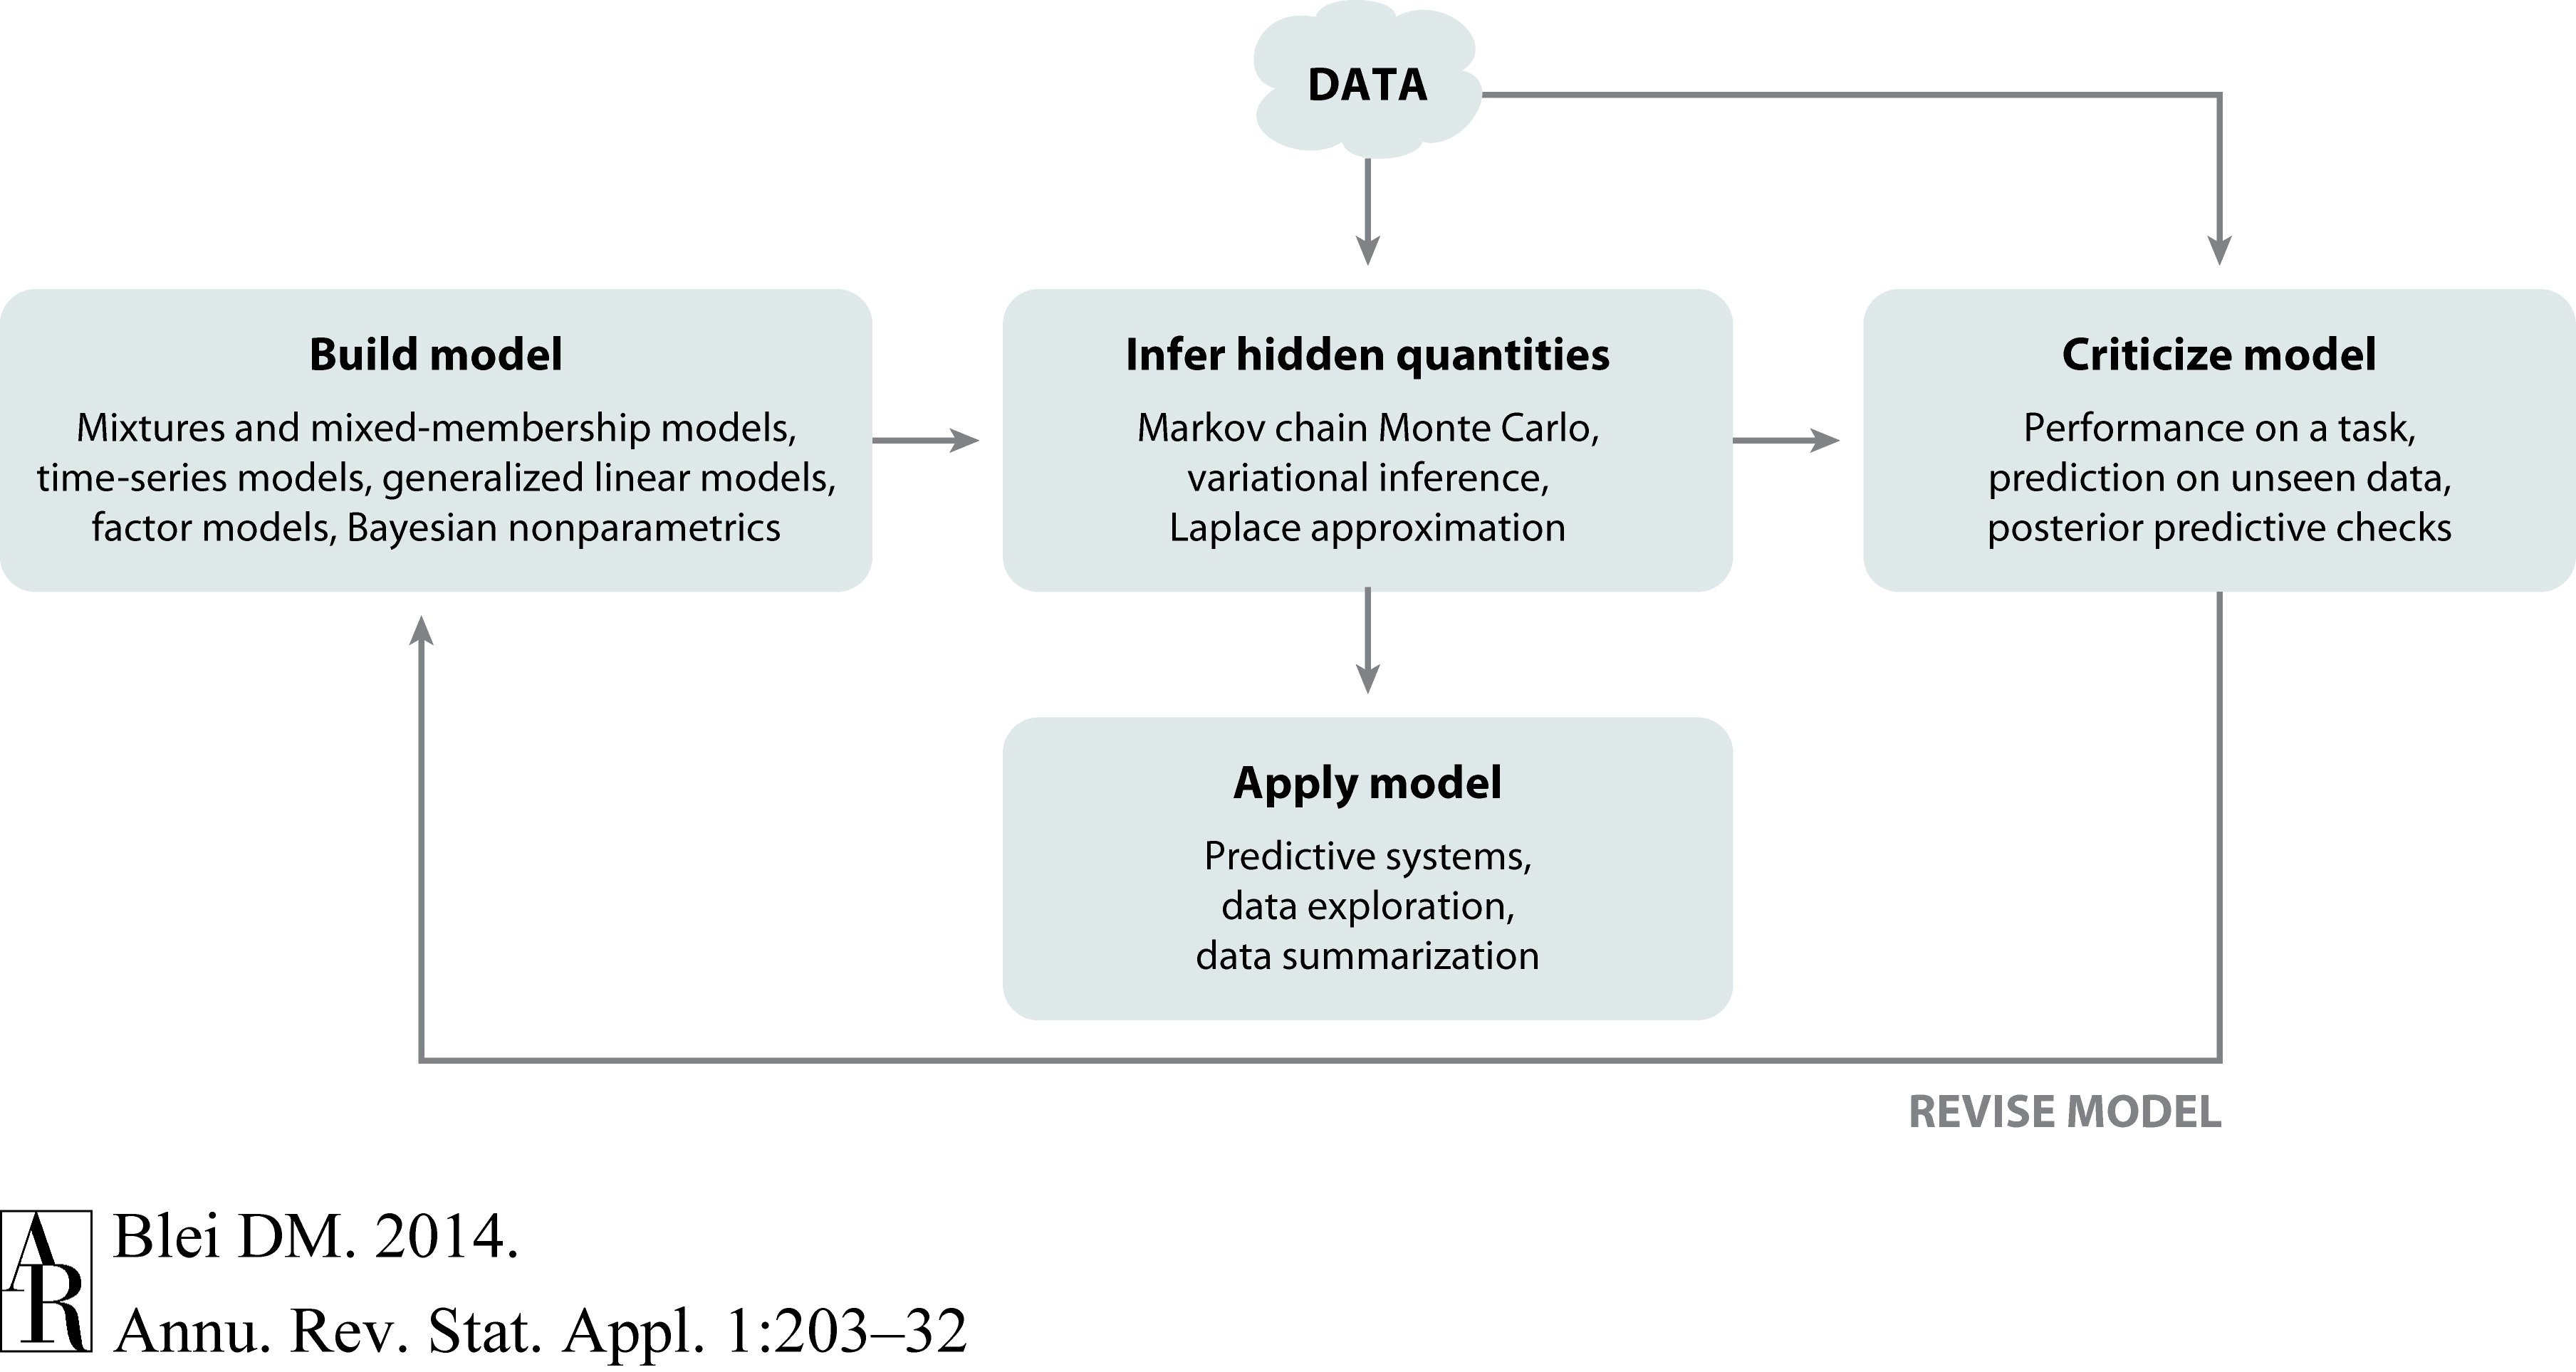
\includegraphics[width=.85\linewidth]{figures/lap1/boxsloop.jpeg}\\
\end{center} 
\begin{flushright}
{\footnotesize Blei, \textit{Ann. Rev. Stat. App.} 2014.}
\end{flushright}
\end{frame}

\begin{frame}{Lap 8: Gaussian processes, elliptical slice sampling, and Bayesian optimization}
\begin{itemize}
    \item \hyperref[sec:gps]{\textbf{Model:} Gaussian processes}
    \item \hyperref[sec:ess]{\textbf{Algorithm:} Elliptical slice sampling}
    \item \hyperref[sec:bopt]{\textbf{Application:} Bayesian optimization}
\end{itemize}
\end{frame}

\section{Model: GPs}
\label{sec:gps}

\begin{frame}{Gaussian processes}
\begin{columns}
\begin{column}{.5\textwidth}
\begin{itemize}
    \item Gaussian processes are distributions on functions~$f: \reals^D \to \reals$. (We can generalize to other domains as well.)
    \item Equivalently, a GP is a continuous set of r.v.'s $\{f(\mbx): \mbx \in \reals^D\}$; i.e. a stochastic process.
\end{itemize}
\end{column}
\begin{column}{.45\textwidth}
\begin{center}
    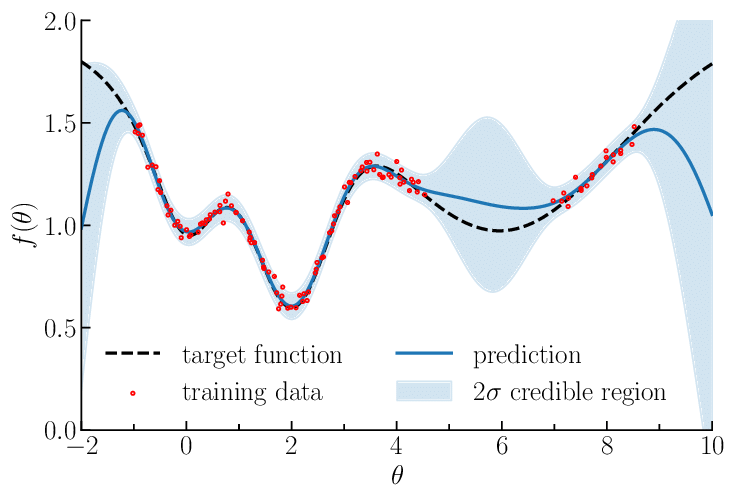
\includegraphics[width=\textwidth]{figures/lap8/gp.png}
    
    \footnotesize{\url{https://www.researchgate.net/figure/Illustration-of-Gaussian-process-regression-in-one-dimension-for-the-target-test_fig1_327613136}}
\end{center}
\end{column}
\end{columns}
\end{frame}


\begin{frame}{Gaussian processes II}

We say $f \sim \distGP(\mu(\cdot), K(\cdot, \cdot))$ if
\begin{align}
    \begin{bmatrix}
    f(\mbx_1) \\ \vdots \\ f(\mbx_N)
    \end{bmatrix} 
    &\sim 
    \cN \left(
    \begin{bmatrix}
    \mu(\mbx_1) \\ \vdots \\ \mu(\mbx_N)
    \end{bmatrix}, \;
    \begin{bmatrix}
    K(\mbx_1, \mbx_1) & \cdots & K(\mbx_1, \mbx_N) \\ 
    \vdots & & \vdots \\ 
    K(\mbx_N, \mbx_1) & \cdots & K(\mbx_N, \mbx_N) 
    \end{bmatrix}
    \right)
\end{align}
for all finite subsets of points $\{\mbx_1, \ldots, \mbx_N\} \subset \reals^D$.

Here, $\mu: \reals^D \to \reals$ is the \textbf{mean function} and $K: \reals^D \times \reals^D \to \reals$ is the \textbf{covariance function}, or \textbf{kernel}.

The covariance matrix obtained by applying the covariance function to each pair of data points above is called the \textbf{Gram matrix}.

The covariance function must be positive definite; i.e. the Gram matrix must be positive definite for any subset of points. 

\end{frame}

\begin{frame}{From linear regression to GPs}
\begin{columns}
\begin{column}{.5\textwidth}
\begin{itemize}
\item Think back to Lap 1: Bayesian Linear Regression. 

\item Our motivating example was approximating a $D=1$ dimensional function $y(x): \reals \to \reals$ given noisy observations $\{y_n, x_n\}_{n=1}^N$. 

\item We cast polynomial regression as linear regression by encoding the inputs $x_n$ with feature vectors,
\begin{align}
    \mbphi(x_n) = (x_n^0, x_n^1, \ldots, x_n^{P-1}) \in \reals^{P}.
\end{align}

\item (I've changed notation slightly to match the slides above.)
\end{itemize}
\end{column}

\begin{column}{0.5\textwidth}
    \centering
    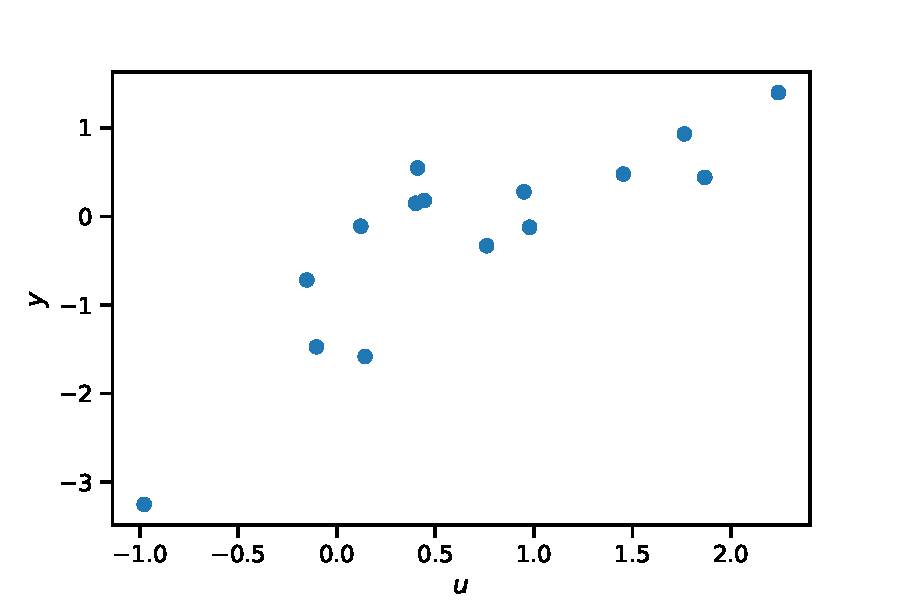
\includegraphics[width=\linewidth]{figures/lap1/data.pdf}
\end{column}
\end{columns}

\end{frame}

\begin{frame}{From linear regression to GPs II}
\label{slide:linreg}
More generally, let $\mbphi(x) = (\phi_1(x), \ldots, \phi_P(x)) \in \reals^P$ be a function that encodes $x$ in a $P$-dimensional feature space. 

With these features, our linear model was,
\begin{align}
    \E[y_n \mid x_n] = \sum_{p=1}^P w_p \phi_p(x_n) = \mbphi(x_n)^\top \mbw &\triangleq f(x_n).
\end{align}

Now assume a Gaussian prior, $\mbw \sim \cN(\mbzero, \tfrac{\lambda}{P} \mbI)$. Then for any $\{x_1, \ldots, x_N\} \subset \reals$,
\begin{align}
    \begin{bmatrix}
    f(x_1) \\ \vdots \\ f(x_N)
    \end{bmatrix} 
    &=
    \begin{bmatrix}
    \phi_1(x_1) & \cdots & \phi_P(x_1) \\ 
    \vdots & & \vdots \\ 
    \phi_1(x_N) & \cdots & \phi_P(x_N) 
    \end{bmatrix}
    \begin{bmatrix}
    w_1 \\ \vdots \\ w_P
    \end{bmatrix}
    = \mbPhi \mbw \sim \cN(\mbzero, \tfrac{\lambda}{P} \mbPhi \mbPhi^\top)
\end{align}
The function $f(\cdot)$ is a GP! It has kernel $K(x_i, x_j) = \tfrac{\lambda}{P} \mbphi(x_i)^\top \mbphi(x_j)$
\end{frame}

% \begin{frame}{From linear regression to GPs III}
% The function values are a linear function of the weights. Since the weights 
% \end{frame}

\begin{frame}{Example: radial basis functions}
Instead of polynomial features, let's use \textbf{radial basis functions},
\begin{align}
    \phi_p(x) = e^{-\frac{1}{2\ell^2}( x-c_p )^2}.
\end{align}
These are un-normalized Gaussian bumps of width $\ell$ located at $c_1,\ldots,c_P$.

With this feature encoding, the kernel is,
\begin{align}
    K(x_i, x_j) = \tfrac{\lambda}{P} \mbphi(x_i)^\top \mbphi(x_j) 
    &= \frac{\lambda}{P} \sum_{p=1}^P e^{-\frac{1}{2\ell^2}(x_i-c_p)^2} e^{-\frac{1}{2\ell^2} (x_j-c_p)^2} 
    % \\
    % &= e^{-\tfrac{1}{2}(x_i^2 + x_j^2)} \sum_{p=1}^P e^{(x_i + x_j)c_p - c_p^2}
\end{align}
Now take the limit of having $P \to \infty$ equally spaced centers. Then,
\begin{align}
    \lim_{P \to \infty} K(x_i, x_j) 
    &= \lambda \int_{-\infty}^\infty e^{-\frac{1}{2\ell^2} (x_i-c)^2} e^{-\frac{1}{2\ell^2} ( x_j-c)^2} \dif c
    % \\
    % &= e^{-(x_i^2 + x_j^2)} \int_{-\infty}^\infty e^{2(x_i + x_j)c - 2c^2} \dif c \\
    % &= 
    = \sqrt{\pi} \ell \lambda e^{-\tfrac{1}{2 (\sqrt{2} \ell)^2} (x_i - x_j)^2}
\end{align}
This is called a \textbf{squared exponential kernel} with length scale $\sqrt{2} \ell$ and variance $\sqrt{\pi} \ell \lambda$.
\end{frame}

\begin{frame}{Demo: sampling GPs with squared exponential kernels}
    
\begin{center}
    \url{https://colab.research.google.com/drive/1PFF5EkD-6g4Ta_4oU3y5ErdzQKh0T1lX?usp=sharing}
\end{center}
    
\end{frame}

\begin{frame}{The Mat\'{e}rn family of kernels}
The Mat\'{e}rn family of kernels is defined by
\begin{align}
    K(x_i, x_j) &= \frac{2^{1-\nu}}{\Gamma(\nu)} \left(\frac{\sqrt{2\nu} \Delta_{ij}}{\ell} \right)^\nu K_\nu \left(\frac{\sqrt{2\nu} \Delta_{ij}}{\ell} \right),
\end{align}
where 
\begin{itemize}
    \item $\Delta_{ij} = x_i - x_j$ is the difference of the points,
    \item $\ell$ is a positive length scale,
    \item the positive parameter $\nu$ controls the smoothness of the function, and 
    \item and $K_\nu$ (in a potentially confusing overloading of notation) denotes the modified Bessel function.
\end{itemize}

When $\nu \to \infty$, the Mat\'{e}rn kernel converges to the squared exponential.

When $\nu = \tfrac{1}{2}$ the kernel is $K(x_i, x_j) = e^{-\frac{\Delta_{ij}}{\ell}}$, the covariance function of the \textbf{Ornstein-Uhlenbeck (OU) process}, a continuous-time AR(1) process.

When $\nu = p - \tfrac{1}{2}$, the kernel is the covariance of a continuous-time AR($p$) process.
\end{frame}

\begin{frame}{The Mat\'{e}rn family of kernels II}
\begin{center}
    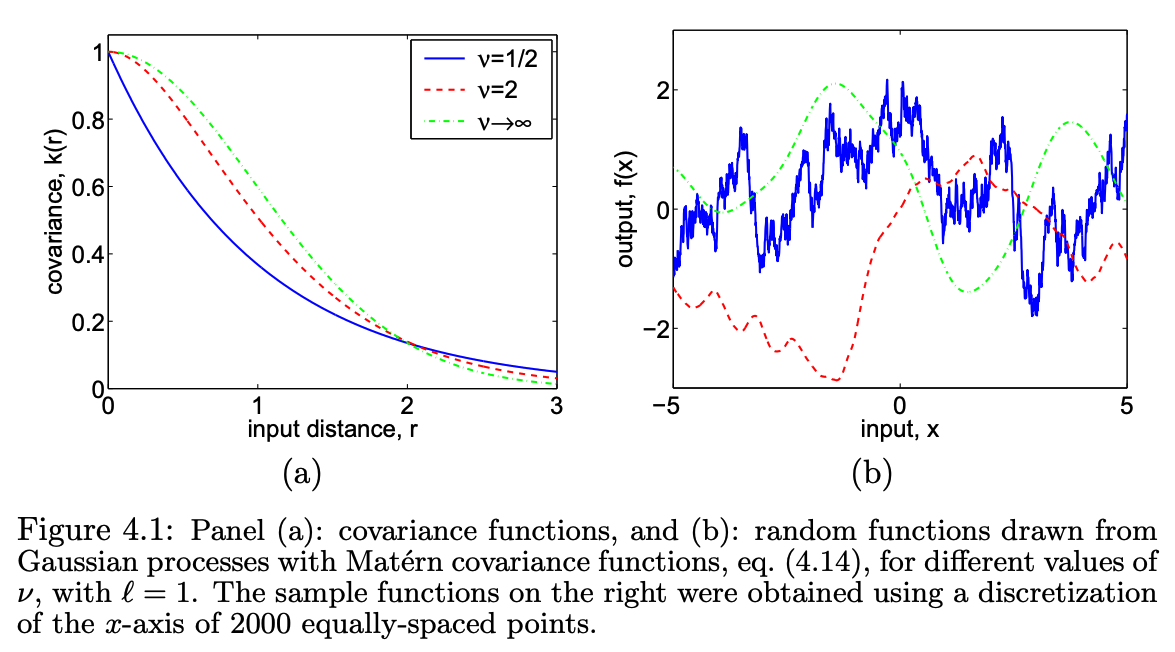
\includegraphics[width=.8\textwidth]{figures/lap8/matern.png}
\end{center}
\end{frame}

\begin{frame}{Stationary kernels and Bochner's theorem}
Note that both the squared exponential and the Mat\'{e}rn kernels are \textbf{stationary} in that $K(\mbx_i, \mbx_j)$ only depends on $\mbDelta_{ij} = \mbx_i - \mbx_j$.

Stationary kernels are particularly interesting because they can be defined by their power spectrum.

\begin{theorem}[Bochner's Theorem]
A complex-valued function $K(\mbDelta)$ on $\reals^D$ is the covariance function of a weakly stationary mean square continuous complex valued random process on $\reals^D$ if and only if it can be represented as 
\begin{align}
    K(\mbDelta) = \int_{\reals^D} e^{2 \pi i \mbs\cdot \mbDelta} \dif \mu(\mbs)
\end{align}
where $\mu$ is a positive finite measure.
\end{theorem}
If $\mu$ has a density $S(\mbs)$ then $S$ is known as the \textbf{spectral density} or \textbf{power spectrum} corresponding to~$K(\mbDelta)$. (This is Theorem 4.1 of~\citet{williams1996gaussian}.)

\end{frame}

\begin{frame}{Power spectrum intuition}
Think of $\mu(\mbs)$ as the power put into frequency $\mbs$. The constraint that it be positive is akin to requiring that the covariance be positive definite.

The \textbf{Wiener-Khintchine theorem} says that covariance function and the spectral density (assuming it exists) are Fourier duals of one another,
\begin{align}
    K(\mbDelta) &= \int S(\mbs) e^{2 \pi i \mbs \cdot \mbDelta} \dif \mbs, \\
    S(\mbs) &= \int K(\mbDelta) e^{-2 \pi i \mbs \cdot \mbDelta} \dif \mbDelta
\end{align}

The variance of the process is $K(\mbzero) = \int S(\mbs) \dif \mbs$ so the spectral density must be integrable (it must decay sufficiently fast as $|\mbs| \to \infty$) to define a valid process.

One nice consequence: the Gram matrix of a stationary kernel evaluated at evenly spaced points $x_1, \ldots, x_N$ in 1D is a \textbf{Toeplitz matrix}, which can be inverted in only $O(N \log N)$ time using the Fourier transform~\citep{Storkey1999-wq,Cunningham2008-zj}
\end{frame}

\begin{frame}{Common kernels}
    \begin{center}
        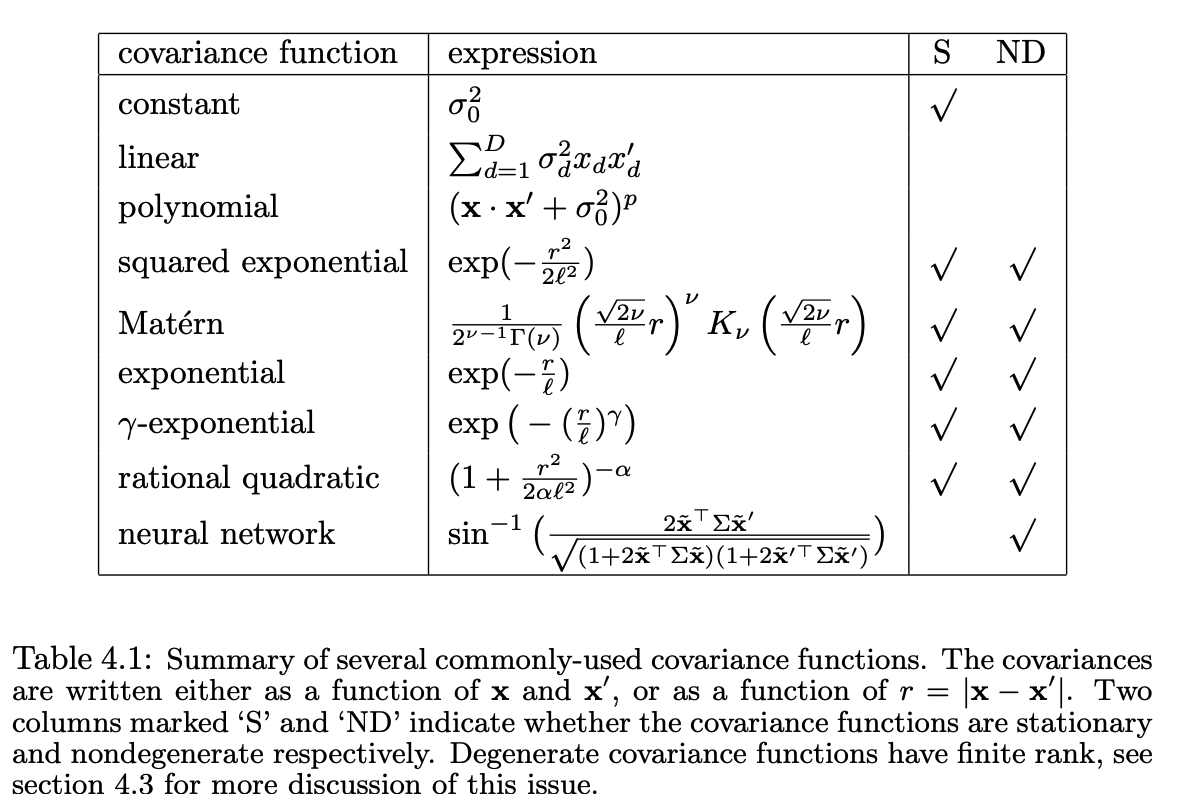
\includegraphics[width=.7\textwidth]{figures/lap8/kernels.png}
    \end{center}
    \vfill
    \hfill From~\citet{williams1996gaussian}
\end{frame}

\begin{frame}{Adding and multiplying kernels}
    \begin{center}
        
\includegraphics[width=.7\textwidth]{figures/lap8/cookbook.png}
        \url{https://www.cs.toronto.edu/~duvenaud/cookbook/}
    \end{center}
\end{frame}

\begin{frame}{The ``Automated Statistician''}
\citet{duvenaud2013structure} proposed a method to search over compositions of kernels to best fit the data. The idea is very cool, but unfortunately they came up with the \textit{worst name ever}.

\begin{center}
    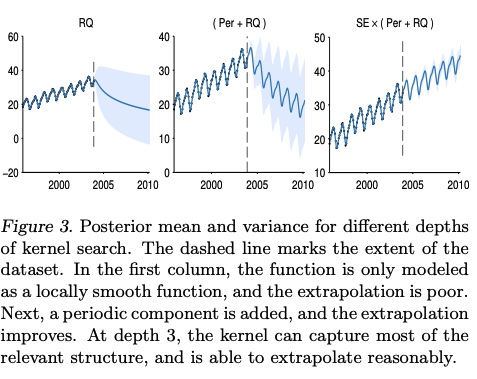
\includegraphics[width=.5\textwidth]{figures/lap8/autostat.png}
\end{center}
\end{frame}

\begin{frame}{Gaussian process regression}
Now that we have a prior distribution on functions, suppose we observe $(y_n, \mbx_n)$ pairs. Assume,
\begin{align}
    f &\sim \distGP(\mu(\cdot), K(\cdot, \cdot)) & y_n & \sim \cN(f(\mbx_n), \sigma^2)
\end{align}
independently for $n=1,\ldots,N$.

Let $\mby = [y_1, \ldots, y_N]^\top$, $\mbmu = [\mu(\mbx_1), \ldots, \mu(\mbx_N)]^\top$, $\mb{f} = [f(\mbx_1), \ldots, f(\mbx_N)]^\top$, and $\mbK$ denote the Gram matrix of $\mbx_1,\ldots, \mbx_N$. Under the GP prior, 
\begin{align}
    p(\mb{f} \mid \{\mbx_n, y_n\}_{n=1}^N) 
    &\propto \left[\prod_{n=1}^N p(y_{n} \mid f(\mbx_n))\right] \, p(\mb{f}) \dif \mb{f} \\
    &= \cN(\mby \mid \mb{f}, \sigma^2 \mbI) \, \cN(\mb{f} \mid \mbmu, \mbK) \dif \mb{f} \\
    &\propto \cN(\mb{f} \mid \mbmu', \mbK'),
\end{align}
where
\begin{align}
    \mbK' &= (\mbK^{-1} + \sigma^{-2} \mbI)^{-1} & 
    \mbmu' &= \mbK'(\mbK^{-1} \mbmu + \sigma^{-2} \mby) 
\end{align}
\end{frame}

\begin{frame}{Marginal distribution}
Likewise, we can integrate over the random function to obtain the marginal distribution,
\begin{align}
    p(\mby) &= \int p(\mby \mid \mb{f}) \, p(\mb{f}) \dif \mb{f} \\
    &= \int \cN(\mby \mid \mb{f}, \sigma^2 \mbI) \, \cN(\mb{f} \mid \mbmu, \mbK) \dif \mb{f} \\
    &= \cN(\mby \mid \mbmu, \mbK + \sigma^2 \mbI).
\end{align}
This allows us to compute the marginal likelihood of the data exactly.

\end{frame}

\begin{frame}{Posterior predictive distribution}
What is the posterior predictive distribution $p(y_{N+1} \mid \mbx_{N+1}, \{\mbx_n, y_n\}_{n=1}^N)$?

It's one big Gaussian model,
\begin{align}
    \begin{bmatrix}
    y_1 \\ \vdots \\ y_N \\ y_{N+1} 
    \end{bmatrix} 
    &\sim 
    \cN \left(
    \begin{bmatrix}
    \mu(\mbx_1) \\ \vdots \\ \mu(\mbx_N) \\ \mu(\mbx_{N+1})
    \end{bmatrix}, \;
    \begin{bmatrix}
    K(\mbx_1, \mbx_1) & \cdots & K(\mbx_1, \mbx_N) & K(\mbx_1, \mbx_{N+1}) \\ 
    \vdots & & \vdots \\ 
    K(\mbx_N, \mbx_1) & \cdots & K(\mbx_N, \mbx_N) & K(\mbx_N, \mbx_{N+1}) \\
    K(\mbx_{N+1}, \mbx_1) & \cdots & K(\mbx_{N+1}, \mbx_N) & K(\mbx_{N+1}, \mbx_{N+1}) \\
    \end{bmatrix}
    + \sigma^2 \mbI
    \right)
\end{align}
We obtain the predictive likelihood via a \textbf{Schur complement},
\begin{align}
    y_{N+1} \mid \mbx_{N+1}, \{\mbx_n, y_n\}_{n=1}^N 
    &\sim
    \cN(m_{N+1}, v_{N+1}) \\
    m_{N+1} &= \mu(\mbx_{N+1}) + \mbk^\top (\mbK + \sigma^2 \mbI)^{-1} (\mby - \mbmu) \\
    v_{N+1} &= K(\mbx_{N+1}, \mbx_{N+1}) - \mbk^\top (\mbK + \sigma^2 \mbI)^{-1} \mbk + \sigma^2.
\end{align}
where $\mbk = [K(\mbx_1, \mbx_{N+1}), \ldots, K(\mbx_N, \mbx_{N+1})]^\top \in \reals^N$.
\end{frame}

\begin{frame}{GPs are linear predictors}
Assume that $\mu(\mbx) = 0$ everywhere.  Then we can write the predictive mean as,
\begin{align}
    m_{N+1} &= \sum_{n=1}^N \alpha_n y_n,
\end{align}
where
\begin{align}
    \alpha_n &= [\mbK^{-1} \mbk]_n
\end{align}

\textbf{Question: } what is the complexity of computing the predictive mean?
\end{frame}

\begin{frame}{Recall the posterior predictive distribution in Bayesian linear regression}
In Bayesian linear regression, we first compute the posterior mean of the weights.

In our notation from Slide~\ref{slide:linreg}, the posterior mean (under an uninformative prior) was,

\begin{align}
    \E[\mbw \mid \{\mbx_n, y_n\}_{n=1}^N] &= \left(\mbPhi^\top \mbPhi + \mbI \right)^{-1} \left(\mbPhi^\top \mby \right)
\end{align}
so the prediction would be
\begin{align}
    \E[y_{N+1} \mid \mbx_{N+1}, \{\mbx_n, y_n\}_{n=1}^N] &= \mbphi(\mbx_{N+1})^\top \left(\mbPhi^\top \mbPhi + \mbI\right)^{-1} \left(\mbPhi^\top \mby \right)
\end{align}

\textbf{Question:} what is the complexity of computing the predictive mean in Bayesian linear regression?

\textbf{Question:} When is it more efficient to work with kernels rather than weights?
\end{frame}

\begin{frame}{GP Classification}
We've seen how Gaussian processes can be used for regression problems with $y_n \in \reals$. What if we have binary observations under the following model,
\begin{align}
    f &\sim \distGP(\mu(\cdot), K(\cdot, \cdot)) &
    y_n &\sim \distBernoulli(\sigma(f(\mbx_n)))
\end{align}
independently for $n=1,\ldots,N$.

This is the GP analog of logistic regression.

As in logistic regression, the posterior is \textit{not} available in closed form. All we know is,
\begin{align}
    p(\mb{f} \mid \{\mbx_n, y_n\}_{n=1}^N)
    &\propto 
    \left[\prod_{n=1}^N \distBernoulli(y_n \mid \sigma(f(\mbx_n))) \right] \, \cN(\mb{f} \mid \mbmu, \mbK) 
\end{align}

Also like logistic regression, we can use a Laplace approximation. But can we do better?

\end{frame}


\section{Algorithm: Elliptical Slice Sampling}
\label{sec:ess}

\begin{frame}{Lap 8: Gaussian processes, elliptical slice sampling, and Bayesian optimization}
\begin{itemize}
    \item \hyperref[sec:gps]{\textbf{Model:} Gaussian processes}
    \item \hyperref[sec:ess]{\textbf{Algorithm: Elliptical slice sampling}}
    \item \hyperref[sec:bopt]{\textbf{Application:} Bayesian optimization}
\end{itemize}
\end{frame}

\begin{frame}{Slice sampling intuition}
    
\end{frame}

\begin{frame}{Slice sampling}
Slice sampling~\citep{Neal2003-zu} is a MCMC algorithm for distributions with intractable normalization constants. 

Suppose we want to sample a posterior distribution,
\begin{align}
    p(\mbtheta \mid \mby) = \frac{p(\mbtheta, \mby)}{p(\mby)}.
\end{align}
Assume we can evaluate the joint probability (numerator) but not the marginal (denominator). 

Slice sampling works by introducing an \textbf{auxiliary variable} $u \in \reals$ so that,
\begin{align}
    p(u, \mbtheta \mid \mby) &= 
    \begin{cases}
    \frac{1}{p(\mby)} & \text{if } 0 \leq u \leq p(\mbtheta, \mby) \\
    0 & \text{o.w.}
    \end{cases}
\end{align}
Note that marginalizing over $u$ recovers the posterior, 
\begin{align}
    \int p(u, \mbtheta \mid \mby) \dif u = \int_0^{p(\mbtheta, \mby)} \frac{1}{p(\mby)} \dif u = \frac{p(\mbtheta, \mby)}{p(\mby)} = p(\mbtheta \mid \mby).
\end{align}
If we can sample $p(u, \mbtheta \mid \mby)$, we can simply throw away the $u$'s to get samples from $p(\mbtheta \mid \mby)$.
\end{frame}

\begin{frame}{Slice sampling II}
    Gibbs sampling is often easy in the augmented space of $(u, \mbtheta)$:
    
    Given $\mbtheta$, the auxiliary variable $u$ follows a uniform distribution,
    \begin{align}
        p(u \mid \mbtheta, \mby) &\propto p(u, \mbtheta \mid \mby) 
        = \frac{1}{p(\mby)} \bbI[0 \leq u \leq p(\mbtheta, \mby)]
        \propto \distUniform(u; [0, p(\mbtheta, \mby)]).
    \end{align}
    
    Given $u$, the variable of interest $\mbtheta$ is uniformly distributed as well,
    \begin{align}
        p(\mbtheta \mid u, \mby) &\propto p(u, \mbtheta \mid \mby) 
        = \frac{1}{p(\mby)} \bbI[p(\mbtheta, \mby) \geq u]
        \propto \distUniform(\mbtheta; \mbTheta(u)),
    \end{align}
    where $\mbTheta(u) = \{\mbtheta': p(\mbtheta', \mby) \geq u\}$ is a \textbf{slice} of parameter space with joint probability at least $u$.
    
    If we can find that slice and sample uniformly from it, we're in business!
    
\end{frame}

\begin{frame}{Slice sampling III}
    $\mbTheta(u)$ is generally a complex subset that is hard to sample uniformly.
    
    Instead, we typically sampling one coordinate of $\mbtheta$ at a time, holding the rest of fixed. (This is also a valid Gibbs update.) 
    
    Still, we need some way of finding the slice. \citet{Neal2003-zu} proposes a ``stepping out'' procedure to compute a 1D slice.
\end{frame}

\begin{frame}[t]{Slice sampling for GPs}
    Consider a GP classification with 2 data points ($\mbx_1$, $\mbx_2$). Assume they are close relative to the length-scale of a squared exponential kernel.
\end{frame}

\begin{frame}{Accounting for the correlated Gaussian prior}

Single variable slice sampling, like all Gibbs sampling methods, suffers when the coordinates are correlated. 

For Gaussian processes, the prior induces correlations between the function values, and this can serious impair such coordinate-wise update algorithms. 

Can we reparameterize the problem so that our 1D slice is better aligned with the prior?
    
\end{frame}

\begin{frame}{A strange way to sample a Gaussian...}

Suppose $\mb{f} \sim \cN(\mbzero, \mbSigma)$. A strange but interesting way to sample $\mb{f}$ is via the following program:
\begin{align}
    \mbnu_0 &\sim \cN(\mbzero, \mbSigma) \\
    \mbnu_1 &\sim \cN(\mbzero, \mbSigma) \\
    \theta &\sim \distUniform([0, 2\pi)) \\
    \mb{f} &= \mbnu_0 \sin \theta + \mbnu_1 \cos \theta
\end{align}
To see this, define $\mbnu' = \begin{bmatrix} \mbnu_0 & \mbnu_1  \end{bmatrix}^\top$ and note that for any $\theta \in [0, 2 \pi)$
\begin{align}
    \mbnu' 
    &\sim 
    \cN \left(
    \begin{bmatrix}
        \mbzero \\ 
        \mbzero 
    \end{bmatrix},
    \begin{bmatrix}
        \mbSigma & \mbzero \\ 
        \mbzero & \mbSigma
    \end{bmatrix}
    \right), \\
    \mb{f} &= 
    \begin{bmatrix} \sin \theta \mbI & \cos \theta \mbI \end{bmatrix} \mbnu' 
    \sim \cN \left(
    \mbzero, 
    \begin{bmatrix} \sin \theta \mbI & \cos \theta \mbI \end{bmatrix}
    \begin{bmatrix}
        \mbSigma & \mbzero \\ 
        \mbzero & \mbSigma
    \end{bmatrix}
    \begin{bmatrix} \sin \theta \mbI \\ \cos \theta \mbI \end{bmatrix}
    \right) \\
    &\sim \cN(\mbzero, (\sin^2 \theta + \cos^2 \theta) \mbSigma) = \cN(\mbzero, \mbSigma).
\end{align}
    
\end{frame}

\begin{frame}{Elliptical slice sampling}
With this sampling procedure in mind, \citet{Murray2010-zb} proposed \textbf{elliptical slice sampling}. 

Reparameterize $\mb{f}$ in terms of $\mbnu_0, \mbnu_1, \theta$ and sample the posterior,
\begin{align}
    p(\mbnu_0, \mbnu_1, \theta \mid \mby) &\propto 
    \cN(\mbnu_0 \mid \mbzero, \mbSigma) \,
    \cN(\mbnu_1 \mid \mbzero, \mbSigma) \,
    \distUniform(\theta \mid [0, 2 \pi)) \,
    p(\mby \mid \mb{f}(\mbnu_0, \mbnu_1, \theta))
\end{align}

Their sampling algorithm consists of two steps:
\begin{enumerate}
    \item Sample $\mbnu_0, \mbnu_1, \theta \mid \mby, \mb{f} = \mbnu_0 \sin \theta + \mbnu_1 \cos \theta$ 
    \begin{enumerate}
        \item Sample $\mbnu \sim \cN(\mbzero, \mbSigma)$ and $\theta \sim \distUniform([0, 2\pi))$. 
        \item Set $\mbnu_0 = \mb{f} \sin \theta + \mbnu \cos \theta$ and $\mbnu_1 = \mb{f} \cos \theta - \mbnu' \sin \theta$.
    \end{enumerate}
    \item Sample $\theta \mid \mbnu_0, \mbnu_1, \mby$ by slice sampling its conditional $p(\theta \mid \mbnu_0, \mbnu_1, \mby) \propto p(\mby \mid \mbnu_0 \cos \theta + \mbnu_1 \sin \theta)$.
\end{enumerate}
We can think of step 2 as slice sampling on an elliptical slice, hence the name. 
\end{frame}

\begin{frame}[t]{Elliptical slice sampling II}
\begin{columns}
\begin{column}{.5\textwidth}
This formulation is a little complicated. There's no need to actually instantiate $\mbnu_0$ and $\mbnu_1$. Instead, we can just work with $\mbnu$ and $\theta$.
\end{column}
\begin{column}{.5\textwidth}
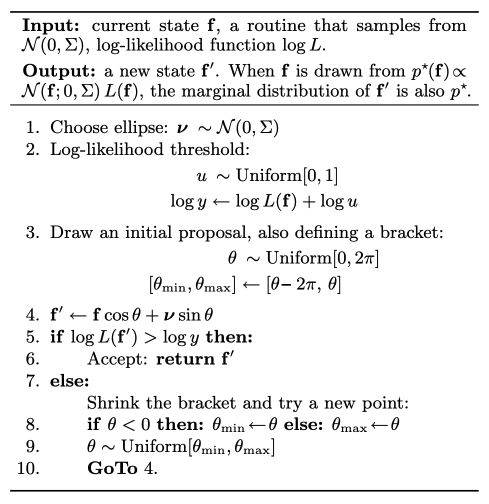
\includegraphics[width=\textwidth]{figures/lap8/ess1.png}
\end{column}
\end{columns}
\end{frame}

\begin{frame}{Elliptical slice sampling III}
    \centering
    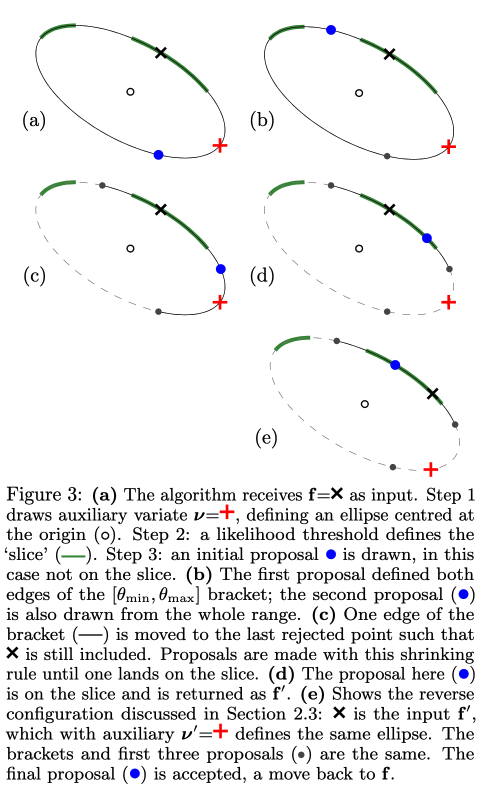
\includegraphics[width=.33\textwidth]{figures/lap8/ess2.png}
\end{frame}

\begin{frame}[t]{Computational complexity}
\textbf{Question: } What is the computational complexity of one elliptical slice sampling update? Assume conditionally independent Bernoulli observations, as in GP classification.
\end{frame}

\section{Sparse GPs}
\label{sec:spgps}

\begin{frame}{Lap 8: Gaussian processes, elliptical slice sampling, and Bayesian optimization}
\begin{itemize}
    \item \hyperref[sec:gps]{\textbf{Model:} Gaussian processes}
    \item \hyperref[sec:ess]{\textbf{Algorithm:} Elliptical slice sampling}
    \item \hyperref[sec:spgps]{\textbf{Algorithm:} Variational Inference with Sparse GPs}
    \item \hyperref[sec:bopt]{\textbf{Application:} Bayesian optimization}
\end{itemize}
\end{frame}


\begin{frame}{Inducing point methods}
The key limitation of GPs is the cubic complexity of inference (with quadratic memory complexity). 

One way of circumventing this complexity is via \textbf{inducing points} \citep{csato2002, snelson2005, tisias2009}. These form the basis of an approximate model called \textbf{Sparse GPs}.

We follow the presentation by \citet{Hensman2013-cf}.
\end{frame}

\begin{frame}{Sparse GPs and Inducing Points}
    Consider a Gaussian process regression with inputs $\{\mbx_n\}_{n=1}^N \subset \reals^D$ and observations $\{y_n\}_{n=1}^N \subset \reals$. As above, let $\mby = [y_1, \ldots, y_N]^\top$ and $\mb{f} = [f(\mbx_1), \ldots, f(\mbx_N)]^\top$
    
    Introduce a set of \textbf{inducing points} $\{\mbz_m\}_{m=1}^M \subset \reals^D$ with corresponding function values $u_m = f(\mbz_m)$.  
    
    Using the GP predictive distribution, we can write,
    \begin{align}
    p(\mby \mid \mb{f}) &= \cN(\mby \mid \sigma^2 \mbI) \\
    p(\mb{f} \mid \mbu) &= \cN(\mb{f} \mid \mbK_{nm} \mbK_{mm}^{-1} \mbu, \, \tilde{\mbK}
    \end{align}
    where $\mbK_{nm}$ is the Gram matrix of kernel evaluations for each $(\mbx_n, \mbz_m)$ pair, $\mbK_{mm}$ is the Gram matrix for each $(\mbz_m, \mbz_m)$ pair, and
    \begin{align}
        \tilde{\mbK} &= \mbK_{nn} - \mbK_{nm} \mbK_{mm}^{-1} \mbK_{mn}.
    \end{align}
    Note that $\tilde{\mbK} \in \reals^{N \times N}$, so we're still looking at $O(N^3)$ complexity.
    
\end{frame}

\begin{frame}{Variational inference for Sparse GPs}
    Now we will lower bound the marginal log likelihood using Jensen's inequality,
    \begin{align}
        \log p(\mby \mid \mbu) &= 
        \log \int p(\mby, \mb{f} \mid \mbu) \dif \mb{f} \\
        \label{eq:bound1} &= \log \E_{p(\mb{f} | \mbu)}[p(\mby \mid \mb{f})] \\
        \label{eq:bound2} &\geq \E_{p(\mb{f} | \mbu)}[\log p(\mby \mid \mb{f})] \\
        &\triangleq \cL_1.
    \end{align}
    Assume $p(\mby \mid \mb{f}) = \prod_{n=1}^N p(y_n \mid f(\mbx_n))$; i.e. the observations are conditionally independent. 
    
    \textbf{Question: } what is the complexity of evaluating the bound in eq.~\eqref{eq:bound2}?
    
    \textbf{Question: } when is the bound maximized?
    
\end{frame}

\begin{frame}{Variational inference for Sparse GPs II}
Using the bound from above, we can obtain a lower bound on the marginal likelihood of the data, integrating out the inducing variables~\citep{Titsias2009-ls},
\begin{align}
    \log p(\mby \mid \mbX) &= 
    \log \int p(\mby \mid \mbu) \, p(\mbu) \dif \mbu \\
    &\geq \log \int \exp\{\cL_1\} \, p(\mbu) \dif \mbu \\
    &\triangleq \cL_2.
\end{align}
After some algebra, this bound equals,
\begin{align}
    \cL_2 &= \log \cN(\mby \mid \mbzero, \mbK_{nm} \mbK_{mm}^{-1} \mbK_{mn} + \sigma^2 \mbI) -\frac{1}{2\sigma^2} \Tr(\tilde{\mbK}).
\end{align}
We can view this bound as arising from a variational approximation $q(\mbu) = \cN(\hat{\mbu}, \mbLambda^{-1})$ where
\begin{align}
    \mbLambda &= \sigma^{-2} \mbK_{mm}^{-1} \mbK_{mn} \mbK_{nm} \mbK_{mm}^{-1} + \mbK_{mm}^{-1} \\
    \hat{\mbu} &= \sigma^{-2} \mbLambda^{-1} \mbK_{mm}^{-1} \mbK_{mn} \mby.
\end{align}
\textbf{Question: } what is the complexity of computing $\cL_2$?
\end{frame}

\begin{frame}{Stochastic variational inference for Sparse GPs}
    Marginalizing over $\mbu$ coupled the observations $\mby$ so that the likelihood was a multivariate Gaussian (albeit with a low rank plus diagonal covariance). 
    
    As we briefly discussed in Lap 5: Mixed Membership Models, if the likelihood factors into a product over data points we can use \textbf{stochastic variational inference}, operating on mini-batches of data instead.
    
    Can we do something similar here?
\end{frame}

\begin{frame}{Stochastic variational inference for Sparse GPs II}
    \citet{Hensman2013-cf} showed that if we explicitly represent $q(\mbu)$, the likelihood $p(\mby \mid \mbu)$ factors into a product over the $N$ data points. 
    
    Define a new lower bound, 
    \begin{align}
        \log p(\mby \mid \mbX) &\geq 
        \E_{q(\mbu)} \left[ \log p(y \mid \mbu) + \log p(\mbu) - \log q(\mbu) \right] \\
        &\geq \E_{q(\mbu)} \left[ \cL_1 + \log p(\mbu) - \log q(\mbu) \right] \\
        &\triangleq \cL_3,
    \end{align}
    and assume $q(\mbu) = \cN(\mbm, \mbS)$.  Then the bound simplifies to,
    \begin{align}
        \cL_3 &= \sum_{n=1}^N \left[ \log \cN(y_n \mid \mbk_n^\top \mbK_{mm}^{-1} \mbm, \, \sigma^2) 
        -\frac{1}{2\sigma^2} \tilde{K}_{n,n} - \frac{1}{2} \Tr(\mbS \mbLambda_{n} \right] 
        - \KL{q(\mbu)}{p(\mbu)}
    \end{align}
    where $\mbk_n$ is the $k$-th column of $\mbK_{mn}$ and $\mbLambda_n = \sigma^{-1} \mbK_{mm}^{-1} \mbk_n \mbk_n^\top \mbK_{mm}^{-1}$.
    
    This lower bound and its gradients wrt $\mbm$ and $\mbS$ can be approximated with Monte Carlo using mini-batches. \citet{Hensman2013-cf} used this trick to fit sparse GPs to millions of data points.
\end{frame}

\begin{frame}[t]{Choosing the inducing points}
    \textbf{Question: } how should we obtain the inducing points?
\end{frame}

\begin{frame}[t,allowframebreaks]
        \frametitle{References}
        \bibliographystyle{unsrtnat}
        \bibliography{refs.bib}
\end{frame}

\end{document}